
\documentclass[a4paper, 12pt]{article}

\usepackage[english, russian]{babel}
\usepackage[T2A]{fontenc}
\usepackage[utf8]{inputenc}
\usepackage{mathtext}
\usepackage{amsfonts}
\usepackage{ amssymb }
\usepackage{amsmath}
\usepackage{graphics}
\usepackage{graphicx}
\usepackage{wrapfig}
\usepackage{geometry}
\usepackage{float}
\geometry{
	a4paper,
	total={170mm, 257mm},
	left=20mm,
	top=10mm}
	
\usepackage{wrapfig}
\usepackage{graphicx}
\usepackage{mathtext}
\usepackage{amsmath}
\usepackage{siunitx} % Required for alignment
\usepackage{subfigure}
\usepackage{multirow}
\usepackage{rotating}
\usepackage{afterpage}
\usepackage[T1,T2A]{fontenc}
\usepackage[russian]{babel}
\usepackage{caption}
\usepackage[arrowdel]{physics}
\usepackage{booktabs}
\usepackage{float}

\graphicspath{{pictures/}}

\title{\begin{center}Лабораторная работа №3.7.1\end{center}
	Скин-эффект в полом цилиндре}
\author{Комкин Михаил, Б01-303}
\date{\today}

\begin{document}
	\maketitle
	\textbf{Цель работы:} Исследование проникновения переменного магнитного поля в медный полый цилиндр
	
	\section*{Теоретическая часть}
	\subsection*{Скин-эффект для полупрастранства}
	\vspace{1cm}
	\begin{wrapfigure}{l}{0.3\textwidth}
		\begin{center}
			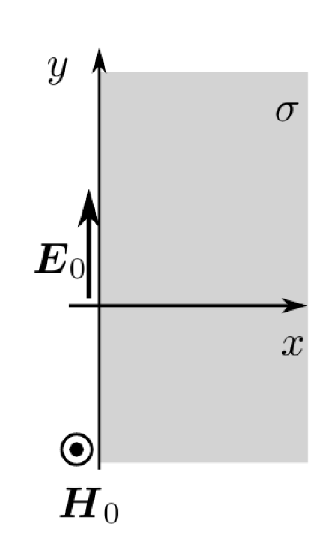
\includegraphics[width=0.28\textwidth]{image}
		\end{center}
		%\caption{Скин-эффект в полупространстве}\label{fig:poluprostranstvo}
	\end{wrapfigure}
	
	Рассмотрим квазистационарное поле внутри проводящей среды в простейшем плоском случае.
	Пусть вектор $\vb*{E}$ направлен всюду вдоль оси $y$ и зависит только от координаты $x$, т. е. ${E_x} = {E_z} \equiv 0$, $E_y=E_y(x,t)$.
	В квазистационарном приближении 
	\begin{equation*}
		\grad \times \vb*{H} = \sigma \vb*{E}
	\end{equation*}
	
	Преобразуя это уравнение, можно получить уравнение, схожее с уравнением диффузии:
	\begin{equation}
		\grad^2\vb*{H}=\sigma\mu\mu_0 \frac{\partial \vb*{H}}{\partial t}\label{eq:laplacian_H}
	\end{equation}
	Точно такое же уравнение имеет место и для вектора $E:$
	\begin{equation}
		\grad^2\vb*{E}=\sigma\mu\mu_0 \frac{\partial \vb*{E}}{\partial t}\label{eq:diffusion}
	\end{equation}
	
	Подставляем в (\ref{eq:diffusion}) наше электрическое поле $E_y=E_y(x,t)$
	\begin{equation}
		\frac{\partial^2 E_y}{\partial x^2} = \sigma\mu\mu_0\frac{\partial E_y}{\partial t}
		\label{eq:diffusion_chastni}
	\end{equation}
	Если $E_y(0,t)=E_0 e^{i\omega t}$ то решением (\ref{eq:diffusion_chastni}) будет функция вида
	\begin{equation}
		E_y(x,t)=E_0 e^{-x/\delta} e^{i(\omega t - x/\delta)}
		\label{eq:skin_effect_poluprostranstvo}
	\end{equation}
	где
	\begin{equation}
		\delta = \sqrt{\frac{2}{\omega\sigma\mu\mu_0}}
		\label{eq:delta}
	\end{equation}
	
	\newpage
	\subsection*{Скин-эффект в тонокм полом цилиндре}
	\vspace{1cm}
	\begin{wrapfigure}[36]{l}{0.3\textwidth}
		\begin{center}
			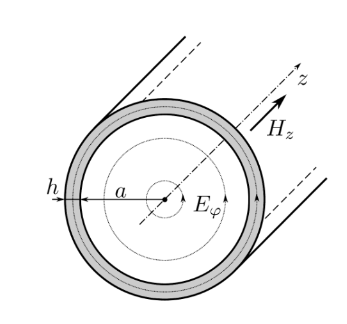
\includegraphics[width=0.28\textwidth]{image2}
		\end{center}
		\caption{Эл-магнитные поля в цилиндре}\label{fig:cilindr}
		
		\begin{center}
			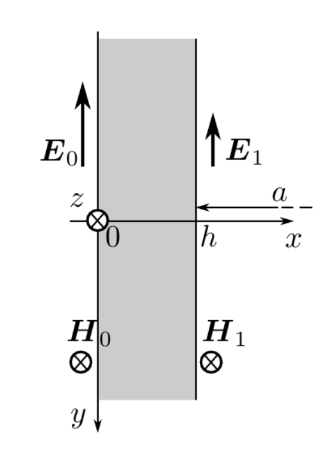
\includegraphics[width=0.28\textwidth]{image3}
		\end{center}
		\caption{Стенка цилиндра}\label{fig:stenka}
	\end{wrapfigure}
	
	Перейдем теперь к описанию теории в нашей работе. Из соображении симметрии и 
	непрерывности соответствующих компонет векторов $\vb*{E}$ и $\vb*{H}$ можем сказать что
	\begin{equation*}
		H_z = H(r)e^{i\omega t} \text{, } E_\varphi = E(r)e^{i\omega t}
	\end{equation*}
	и при этом функции $H(r)$ и $E(r)$ непрерывны.
	
	Внутри цилиндра токов нет, следовательно $H(r)=H_1=\text{const}$ внутри цилиндра.
	По теореме об электромагнитной индукции
	\begin{equation*}
		E(r) = -\frac{1}{2}\mu_0 r \cdot i \omega H_1
	\end{equation*}
	откуда мы получаем граничное условие
	\begin{equation}
		E_1=E(a)= -\frac{1}{2}\mu_0 a \cdot i \omega H_1
		\label{eq:granichnoe_uslovie_E}
	\end{equation}
	
	В прближении $h \ll a$ можем пренебречь кривизной стенки и смоделировать 
	его бесконечной полосой. Тогда, надо решить уравнение (\ref{eq:laplacian_H})
	с граничными условиями. Решая уравнение получим связь полей $H_1$ 
	(поле внутри цилиндра которое мы будем измерять) и $H_0$, которое колебается с частотой
	$\omega$
	
	\begin{equation}
		H_1 = \frac{H_0}{\ch(\alpha h) + \frac{1}{2} \alpha a \sh(\alpha h)} 
		\text{\ \ \ }
		\alpha = \sqrt{i\omega \sigma \mu_0} = \frac{\sqrt{2}}{\delta}e^{i\pi/4}
		\label{eq:svyaz_poley}
	\end{equation}
	
	из этой формулы получим сколько по фазе отстает поле $H_1$ от $H_0$. При $\delta \ll h$
	(высокачастотная область)
	
	\begin{equation}
		\psi \approx \frac{\pi}{4} + \frac{h}{\delta} = 
		\frac{\pi}{4} + h \sqrt{\frac{\omega \sigma \mu_0}{2}}
		\label{eq:faza_high_freq}
	\end{equation}
	
	При $\delta \gg h$ (низкочастотная область)
	
	\begin{equation}
		\tg \psi \approx \frac{ah}{\delta^2} = \pi a h \sigma \mu \mu_0 \nu
		\label{eq:faza_low_freq}
	\end{equation}
	
	\subsection*{Установка и процесс измерения}
	\begin{wrapfigure}{l}{0.4\textwidth}
		\begin{center}
			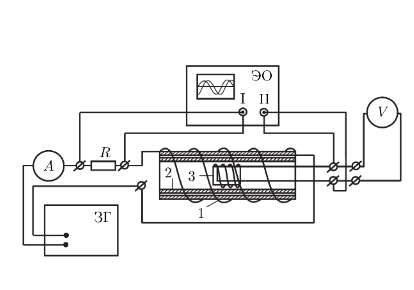
\includegraphics[width=0.38\textwidth]{ustanovka.png}
		\end{center}
		\caption{Установка}\label{fig:ustanovka}
	\end{wrapfigure}
	
	Переменное магнитное поле создается соленоидом 1, на который подается переменный ток со звукового генератора ЗГ. Внутри соленоида расположен медный экран 2. Магнитное поле внутри цилиндра измеряется катушкой 3. Напряжение на катушке пропорциональна производной $\dot{B_1}(t)$
	\begin{equation*}
		U(t) \propto \dot{B_1}(t) = -i\omega H_1 e^{i\omega t}
	\end{equation*}
	Поле внутри цилиндра пропорциональна току через соленоид
	\begin{equation*}
		H_0(t) \propto I(t)
	\end{equation*}
	Отсюда несложно увидеть, что
	\begin{equation}
		\frac{\abs{H_1}}{\abs{H_0}} = c \cdot \frac{U}{\nu I} = \xi_0 \xi
		\label{eq:otnoshenie_amplitud}
	\end{equation}
	где константу  $\xi_0$ можно определить из условия $\abs{H_1}/\abs{H_0} \rightarrow 1$ при
	$\nu \rightarrow 0$.\\
	
	При измерениях разности фаз нужно учесть, что первый сигнал на осциллографе
	пропорционален магнитному полю снаружи, а второй пропорционален производному
	поля внутри цилиндра по времени, поэтому измеренная на осциллографе разность фаз $\varphi$ будет на $\frac{\pi}{2}$ больше реальной $\psi$:
	\[\varphi = \psi + \frac{\pi}{2}\]
\section{Ход работы}
Параметры нашей установки $2a = 45$ мм, $h=1.5$ мм. Проводимость порядка
$\sigma \sim 5\cdot 10^7$ См/м. Получаем оценку для частоты, при которой
глубина проникновения равна толщине стенок цилиндра $\nu_h = 2300$ Гц.

\section{Измерения амплитуд в области низких частот}
В области низких частот толщина скин-слоя превосходит толщину образца $ \delta \gg h$  и из (\ref{eq:svyaz_poley}) получаем
\begin{equation*}
	\left(\frac{|H_1|}{|H_0|}\right)^2 = (\xi_0\xi)^2 \approx \frac{1}{1+\left(\frac{ah}{\delta^2}\right)^2} = \frac{1}{1 + \left(\pi ah\nu\mu_0\sigma\right)^2}
\end{equation*}
Тогда: 
\begin{equation*}
	\frac{1}{\xi^2}=\xi_0^2B^2\nu^2 + \xi_0^2 \text{, где } B=\pi a h \sigma \mu_0
	\label{eq:liniya_dlya_c}
\end{equation*}
\begin{table}[!ht]
    \centering
    \begin{tabular}{|l|l|l|l|l|l|}
    \hline
        $f$, Гц  & $U$, В & $I$, мА & $\xi$  & $\frac{1}{\xi^2}$ & $f^2, \text{Гц}^2$  \\ \hline
        30 & 0.2116 & 459.02 & 0.01536607 & 4235.204642 & 900 \\ \hline
        35 & 0.2441 & 456.7 & 0.015271044 & 4288.076781 & 1225 \\ \hline
        40 & 0.2755 & 454.05 & 0.015169034 & 4345.944104 & 1600 \\ \hline
        50 & 0.3349 & 448.12 & 0.014946889 & 4476.085444 & 2500 \\ \hline
        60 & 0.3891 & 441.47 & 0.01468956 & 4634.281731 & 3600 \\ \hline
        70 & 0.4381 & 434.43 & 0.014406398 & 4818.248448 & 4900 \\ \hline
        75 & 0.466 & 430.8 & 0.014422779 & 4807.309492 & 5625 \\ \hline
        80 & 0.4819 & 427.19 & 0.014100868 & 5029.308509 & 6400 \\ \hline
        85 & 0.502 & 423.61 & 0.013941792 & 5144.732809 & 7225 \\ \hline
        90 & 0.5208 & 420.05 & 0.013776138 & 5269.204401 & 8100 \\ \hline
        100 & 0.5553 & 413.19 & 0.013439338 & 5536.614139 & 10000 \\ \hline
        115 & 0.5996 & 403.5 & 0.012921718 & 5989.071673 & 13225 \\ \hline
    \end{tabular}
\end{table}
\begin{figure}[h!]
	\centering
	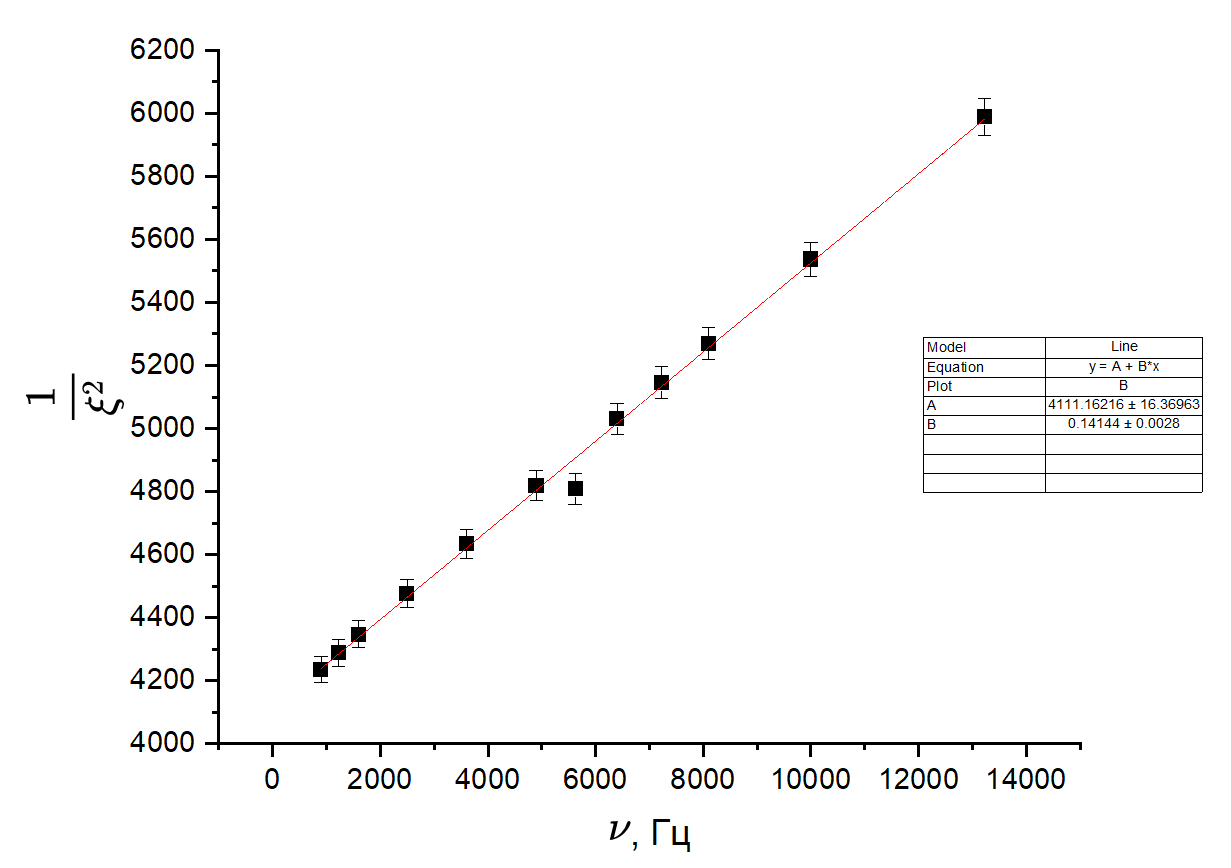
\includegraphics[width=0.9\textwidth, height = 0.45\textheight]{xi(nu).png}
	\caption{График зависимости $1/\xi^2(\nu^2)$}\label{fig:xi_nu_low_freq_linearized}
\end{figure}

Получаем следующие значения: $\xi_0^2B^2 = 0.138, \ \xi_0^2 = 4212.65$, тогда:
\[\xi_0 = 64.11 \pm 4 \ \frac{\text{Гц}}{\text{Ом}}, \ \sigma = (4.38 \pm 0.17) \cdot 10^7 \ \frac{\text{См}}{\text{м}}  \]

\section{Измерение проводимости через разность фаз в низкочастотном диапазоне}
Согласно формуле (\ref{eq:faza_low_freq}), при $\delta \gg h$
\begin{equation*}
    \tan \psi = k \cdot \nu \ \text{; } k = \pi a h \sigma \mu_0 \ \ (\mu = 1)
\end{equation*}
	\begin{figure}[h]
		\center{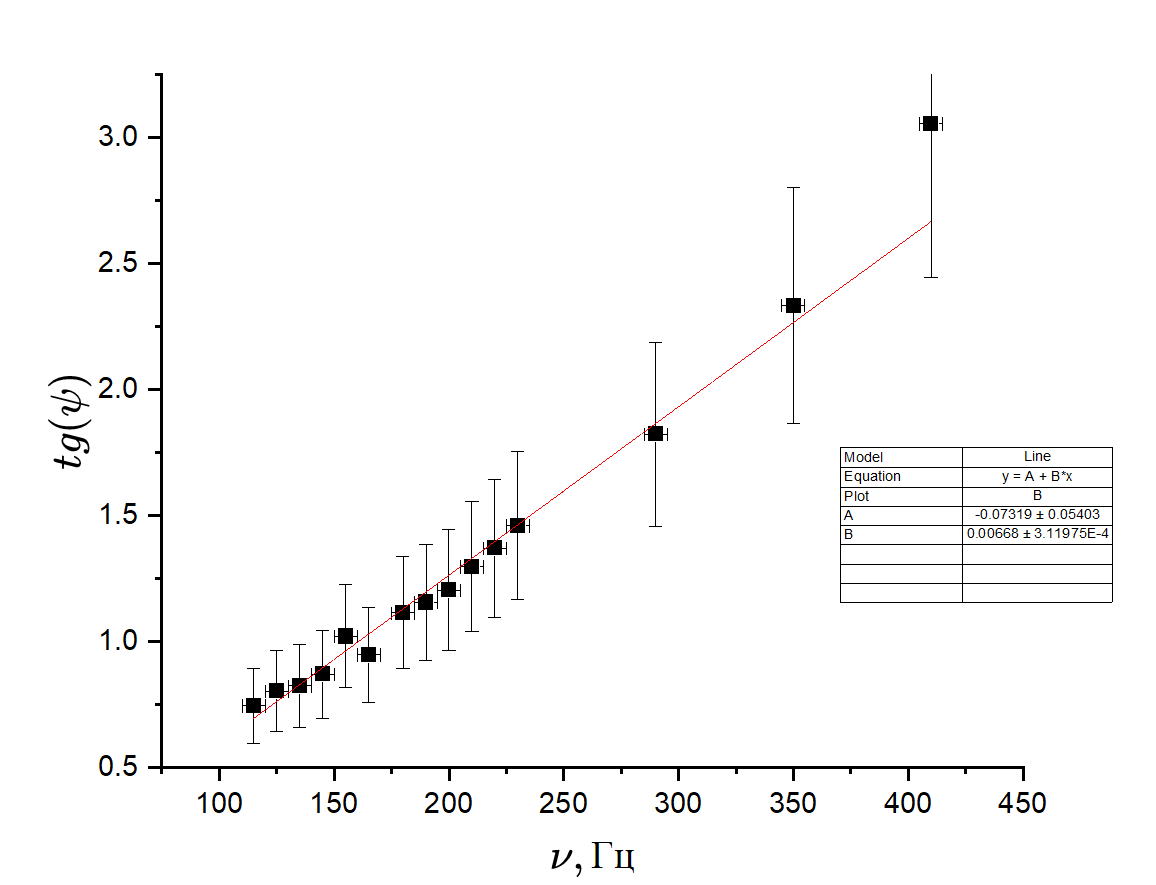
\includegraphics[width=\textwidth]{lin.png}}
		\caption{График зависимости $\tan \psi (\nu)$ (линейная часть)}\label{fig:tg_psi_nu_line}
		\newpage
	\end{figure}
	
	\vspace{1cm}
	Из коэффициента наклона прямой находим проводимость
	\begin{equation}
		\sigma = (4.74 \pm 0.23) \cdot 10^7 \text{См/м}
	\end{equation}
	
	\newpage
	\begin{table}[!ht]
		\centering
		\begin{tabular}{|l|l|l|l|l|l|l|l|}
		\hline
			$f$ & $I$, мА & $U$, В & $x_0$, см & $\Delta x$, см & $\psi, ^\circ$ & $tg(\psi)$ & $\varepsilon_{tg(\psi)}$ \\ \hline
			115 & 416.63 & 549.9 & 3.1 & 4.4 & 2.21 & 0.74 & 0.14 \\ \hline
			125 & 409.57 & 572.4 & 5.8 & 8.1 & 2.24 & 0.80 & 0.16 \\ \hline
			135 & 404 & 593.1 & 5.4 & 7.5 & 2.26 & 0.82 & 0.16 \\ \hline
			145 & 398.87 & 611.2 & 5.1 & 7 & 2.28 & 0.87 & 0.17 \\ \hline
			155 & 394.08 & 627.2 & 4.9 & 6.5 & 2.36 & 1.02 & 0.20 \\ \hline
			165 & 389.63 & 641.2 & 4.6 & 6.2 & 2.32 & 0.94 & 0.18 \\ \hline
			180 & 383.57 & 659.2 & 4.3 & 5.6 & 2.41 & 1.11 & 0.22 \\ \hline
			190 & 379.9 & 669.5 & 4.1 & 5.3 & 2.42 & 1.15 & 0.23 \\ \hline
			200 & 376.5 & 678.5 & 3.9 & 5 & 2.44 & 1.20 & 0.24 \\ \hline
			210 & 373.36 & 686.4 & 3.8 & 4.8 & 2.48 & 1.29 & 0.25 \\ \hline
			220 & 370.44 & 693.6 & 3.6 & 4.5 & 2.51 & 1.37 & 0.27 \\ \hline
			230 & 367.76 & 699.9 & 3.4 & 4.2 & 2.54 & 1.46 & 0.29 \\ \hline
			290 & 354.98 & 725.1 & 7.4 & 8.8 & 2.64 & 1.82 & 0.36 \\ \hline
			350 & 345.97 & 736.9 & 6.8 & 7.8 & 2.73 & 2.33 & 0.46 \\ \hline
			410 & 339.06 & 741.5 & 5.4 & 6 & 2.82 & 3.05 & 0.61 \\ \hline
			470 & 333.24 & 741.9 & 4.9 & 5.1 & 3.01 & 7.92 & 1.58 \\ \hline
			530 & 328.06 & 739.5 & 8.8 & 9.5 & 2.90 & 4.19 & 0.83 \\ \hline
			590 & 323.21 & 735.2 & 8 & 8.5 & 2.95 & 5.28 & 1.05 \\ \hline
			650 & 318.56 & 729.3 & 7.3 & 7.7 & 2.97 & 5.98 & 1.19 \\ \hline
			710 & 313.95 & 722.3 & 6.9 & 7.1 & 3.05 & 10.97 & 2.19 \\ \hline
			770 & 309.35 & 714.5 & 6.3 & 6.6 & 2.99 & 6.84 & 1.36 \\ \hline
			830 & 304.77 & 706 & 5.9 & 6.1 & 3.03 & 9.45 & 1.89 \\ \hline
			890 & 300.21 & 696.9 & 5.55 & 5.7 & 3.05 & 11.73 & 2.34 \\ \hline
			950 & 295.6 & 687.4 & 5.2 & 5.3 & 3.08 & 16.20 & 3.24 \\ \hline
			1010 & 290.99 & 677.6 & 5.9 & 6 & 3.08 & 18.25 & 3.65 \\ \hline
		\end{tabular}
	\end{table}
	\begin{figure}[h]
		\center{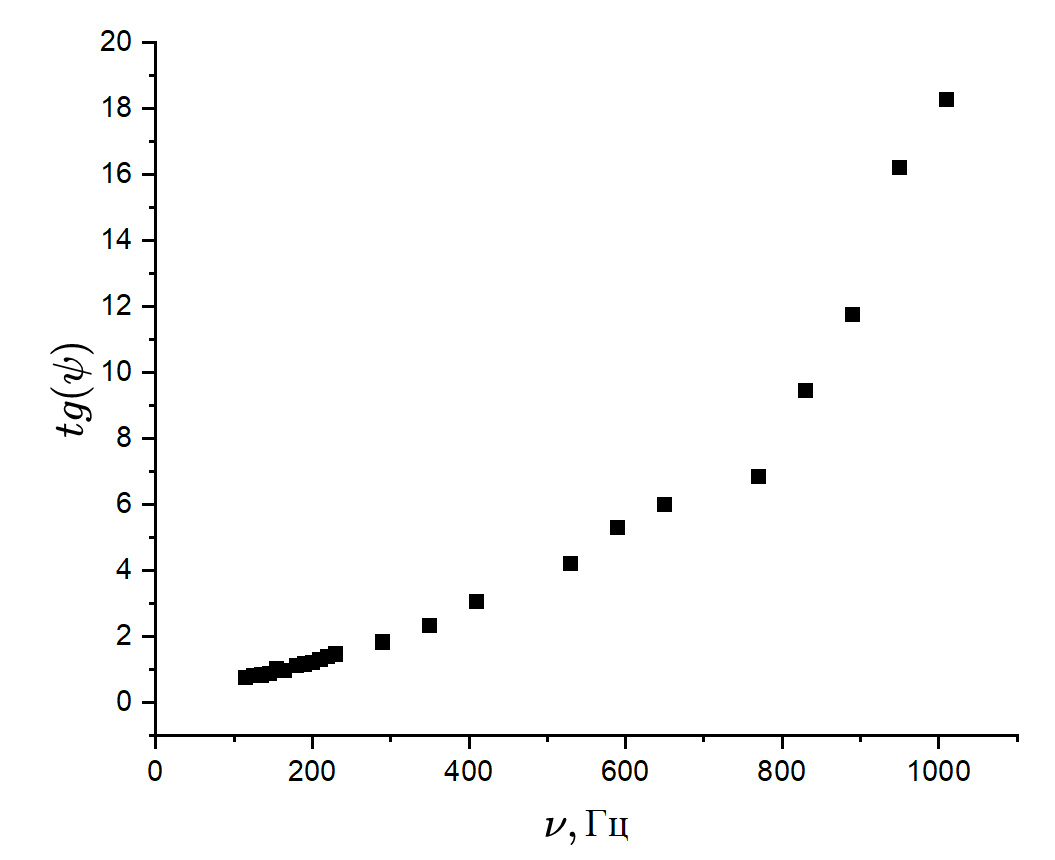
\includegraphics[width=\textwidth]{nonlin.png}}
		\caption{График зависимости $\tan \psi (\nu)$ (нелинейная часть)}\label{fig:tg_psi_nu_no_line}
		\newpage
	\end{figure}
\newpage
	\subsection{Измерение проводимости через разность фаз в высокачастотном диапазоне}
Согласно формуле (\ref{eq:faza_high_freq}), при $\delta \ll h$
\begin{equation*}
    \psi - \pi/4 = k\cdot \sqrt{\nu}; \ k = h\sqrt{\pi\mu_0\sigma}
\end{equation*}
\newpage
\begin{table}[!ht]
    \centering
    \begin{tabular}{|l|l|l|l|l|l|l|l|l|}
    \hline
        $f$, Гц & $I$, мА & $U$, В & $x_0$, см & $\Delta x$, см& $\psi, ^{\circ}$  & $\psi-\pi/4, ^{\circ}$ & $\sqrt{\nu}, \sqrt{\text{Гц}}$ & $\varepsilon{\psi-\pi/4}$ \\ \hline
        1070 & 286.37 & 667.6 & 4.6 & 4.6 & 3.14 & 0.785 & 32.71085447 & 0.0785 \\ \hline
        1130 & 281.71 & 657.3 & 4.2 & 4.2 & 3.14 & 0.785 & 33.61547263 & 0.0785 \\ \hline
        1337 & 265.94 & 621.1 & 7.7 & 7.6 & 3.181315789 & 0.826315789 & 36.5650106 & 0.082631579 \\ \hline
        1588 & 247.27 & 577.5 & 6.6 & 6.4 & 3.238125 & 0.883125 & 39.84971769 & 0.0883125 \\ \hline
        1882 & 226.93 & 529.2 & 5.6 & 5.4 & 3.256296296 & 0.901296296 & 43.38202393 & 0.09012963 \\ \hline
        2231 & 205.33 & 477.4 & 4.9 & 4.6 & 3.344782609 & 0.989782609 & 47.23346271 & 0.098978261 \\ \hline
        2645 & 183.3 & 424 & 4.2 & 3.8 & 3.470526316 & 1.115526316 & 51.42956348 & 0.111552632 \\ \hline
        3135 & 161.67 & 371.1 & 8.8 & 8 & 3.454 & 1.099 & 55.99107072 & 0.1099 \\ \hline
        3716 & 141.08 & 320.5 & 7.6 & 6.7 & 3.561791045 & 1.206791045 & 60.95900262 & 0.120679104 \\ \hline
        4405 & 122.01 & 273.2 & 6.6 & 5.7 & 3.635789474 & 1.280789474 & 66.37017402 & 0.128078947 \\ \hline
        5521 & 99.47 & 216.9 & 5.5 & 4.5 & 3.837777778 & 1.482777778 & 74.30343195 & 0.148277778 \\ \hline
        6189 & 89.31 & 191.3 & 10.2 & 8.2 & 3.905853659 & 1.550853659 & 78.67019766 & 0.155085366 \\ \hline
        7337 & 75.67 & 157 & 7.8 & 5.9 & 4.151186441 & 1.796186441 & 85.6562899 & 0.179618644 \\ \hline
        8697 & 63.8 & 127.1 & 7.7 & 5.9 & 4.097966102 & 1.742966102 & 93.25770746 & 0.17429661 \\ \hline
        10309 & 53.3 & 101.4 & 6.8 & 4.9 & 4.35755102 & 2.00255102 & 101.5332458 & 0.200255102 \\ \hline
        12220 & 43.643 & 79 & 7 & 5.1 & 4.309803922 & 1.954803922 & 110.5441088 & 0.195480392 \\ \hline
        14485 & 35.57 & 61.7 & 5.3 & 3.5 & 4.754857143 & 2.399857143 & 120.3536456 & 0.239985714 \\ \hline
        17170 & 28.237 & 47.8 & 9.4 & 6 & 4.919333333 & 2.564333333 & 131.0343466 & 0.256433333 \\ \hline
        20353 & 21.464 & 37.1 & 8.4 & 5.1 & 5.171764706 & 2.816764706 & 142.6639408 & 0.281676471 \\ \hline
        24126 & 15.043 & 29.3 & 7.4 & 4.4 & 5.280909091 & 2.925909091 & 155.3254648 & 0.292590909 \\ \hline
        28599 & 8.764 & 22.7 & 6.5 & 3.6 & 5.669444444 & 3.314444444 & 169.1123887 & 0.331444444 \\ \hline
        33900 & 2.8591 & 13.9 & 6.4 & 3.1 & 6.482580645 & 4.127580645 & 184.1195264 & 0.412758065 \\ \hline
    \end{tabular}
	
\end{table}
\newpage
Из графика получаем следующее значение проводимости
\begin{figure}[h]
    \center{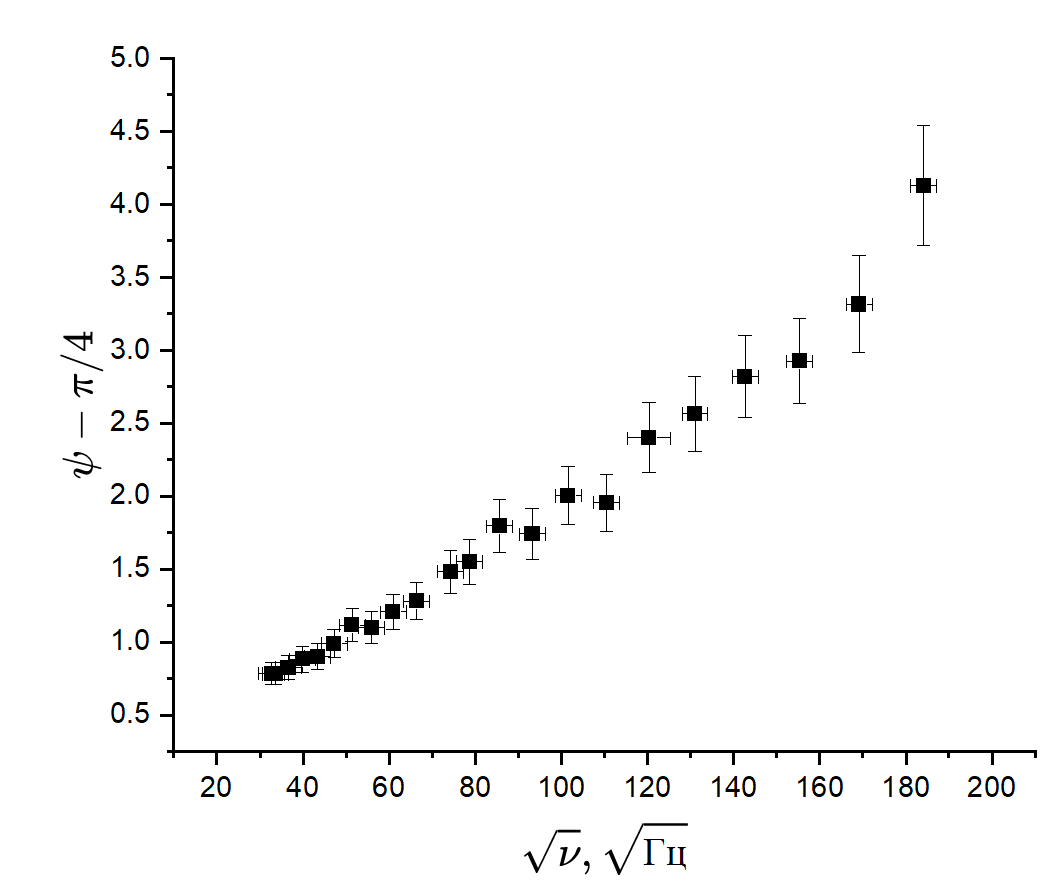
\includegraphics[width=0.9\textwidth]{graph.png}}
    \caption{График зависимости $(\psi - \pi/4)(\sqrt{\nu})$(без аппроксимации)}\label{fig:psi_sqrt_nu}
    \newpage
\end{figure}
\begin{figure}[h]
    \center{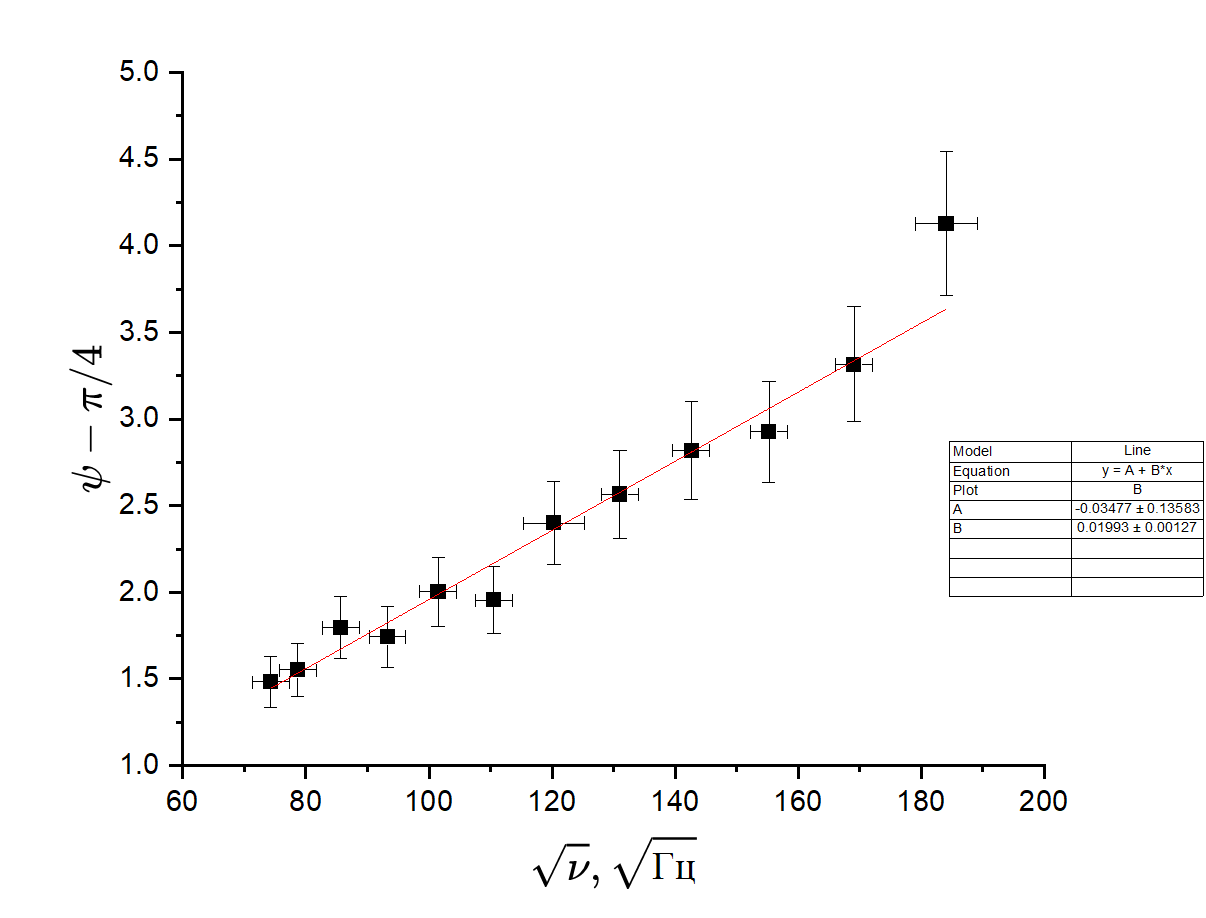
\includegraphics[width=0.9\textwidth]{ghaph2.png}}
    \caption{График зависимости $(\psi - \pi/4)(\sqrt{\nu})$(с аппроксимацией)}\label{fig:psi_sqrt_nu}
    \newpage
\end{figure}
\begin{equation}
    \sigma = (4.28 \pm 0.33) \cdot 10^7 \text{См/м}
\end{equation}
\newpage
\newpage
\subsection{Измерение проводимости через изменение индуктивности}

Из за наличия цилиндра внутри, индуктивность внешней катушки зависит от катушки
следующим образом

\begin{equation*}
    \frac{L_{\max} - L}{L - L_{\min}} = \pi ^2 a^2 h^2 {\mu_0}^2 \sigma^2 \nu^2
\end{equation*}
\newpage
\begin{table}[!ht]
    \centering
    \begin{tabular}{|l|l|l|l|}
    \hline
        $\nu$, Гц & $L$, мГ & ${\nu}^2, \text{Гц}^2$ & $\frac{L_{max} - L_{min}}{L-L_{min}}$ \\ \hline
        40 & 12.3 & 0.0016 & 1 \\ \hline
        100 & 8.6868 & 0.01 & 1.622128861 \\ \hline
        200 & 6.2125 & 0.04 & 2.826158692 \\ \hline
        300 & 4.823 & 0.09 & 4.846193416 \\ \hline
        400 & 4.1035 & 0.16 & 7.693752552 \\ \hline
        500 & 3.7053 & 0.25 & 11.40142805 \\ \hline
        600 & 3.60369 & 0.36 & 13.0000414 \\ \hline
        750 & 3.2618 & 0.5625 & 24.6107628 \\ \hline
        800 & 3.2125 & 0.64 & 28.24887556 \\ \hline
        1000 & 3.09 & 1 & 44.6492891 \\ \hline
        1500 & 2.9612 & 2.25 & 114.6107056 \\ \hline
        10000 & 2.9515 & 100 & 129.9448276 \\ \hline
        15000 & 3.165 & 225000 & 32.94055944 \\ \hline
        20000 & 3.595 & 400000 & 13.15782123 \\ \hline
        25000 & 3.473 & 625000 & 15.86026936 \\ \hline
    \end{tabular}
\end{table}
\begin{figure}[h]
    \center{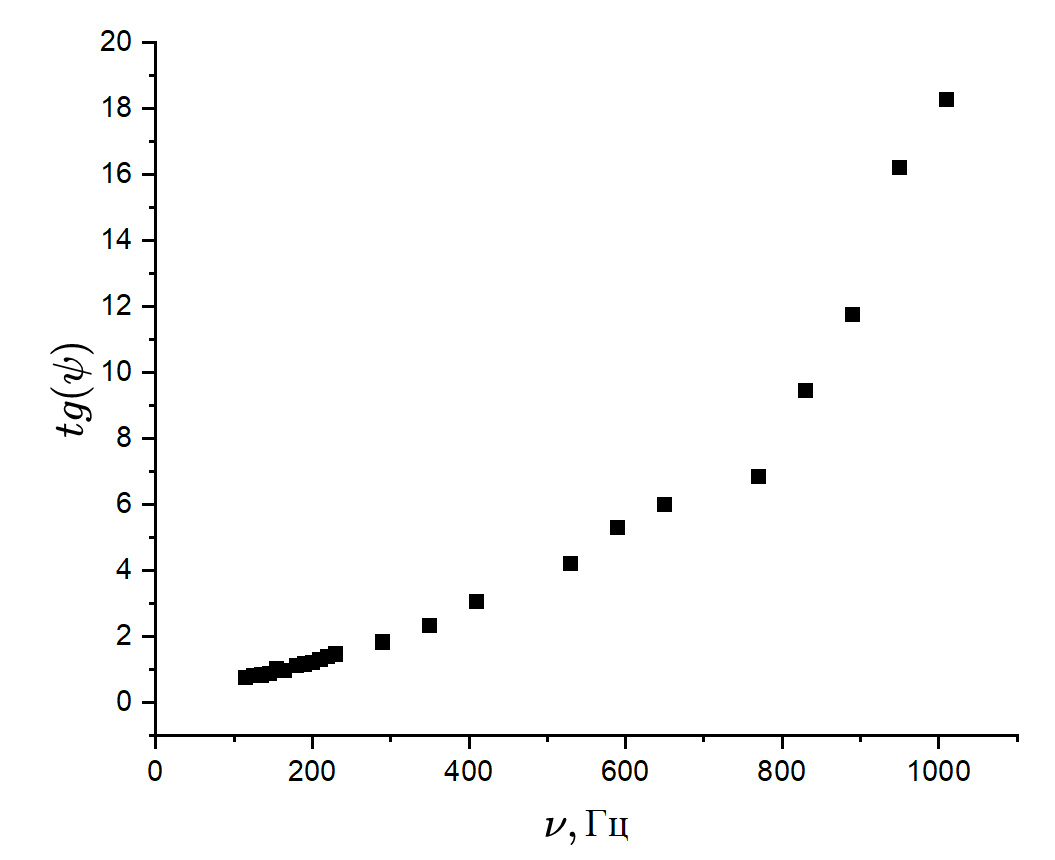
\includegraphics[width=0.7\textwidth]{nonlin.png}}
    \caption{График зависимости $L(\nu)$}\label{fig:L_nu}
    \newpage
\end{figure}

\newpage

\begin{figure}[h]
    \center{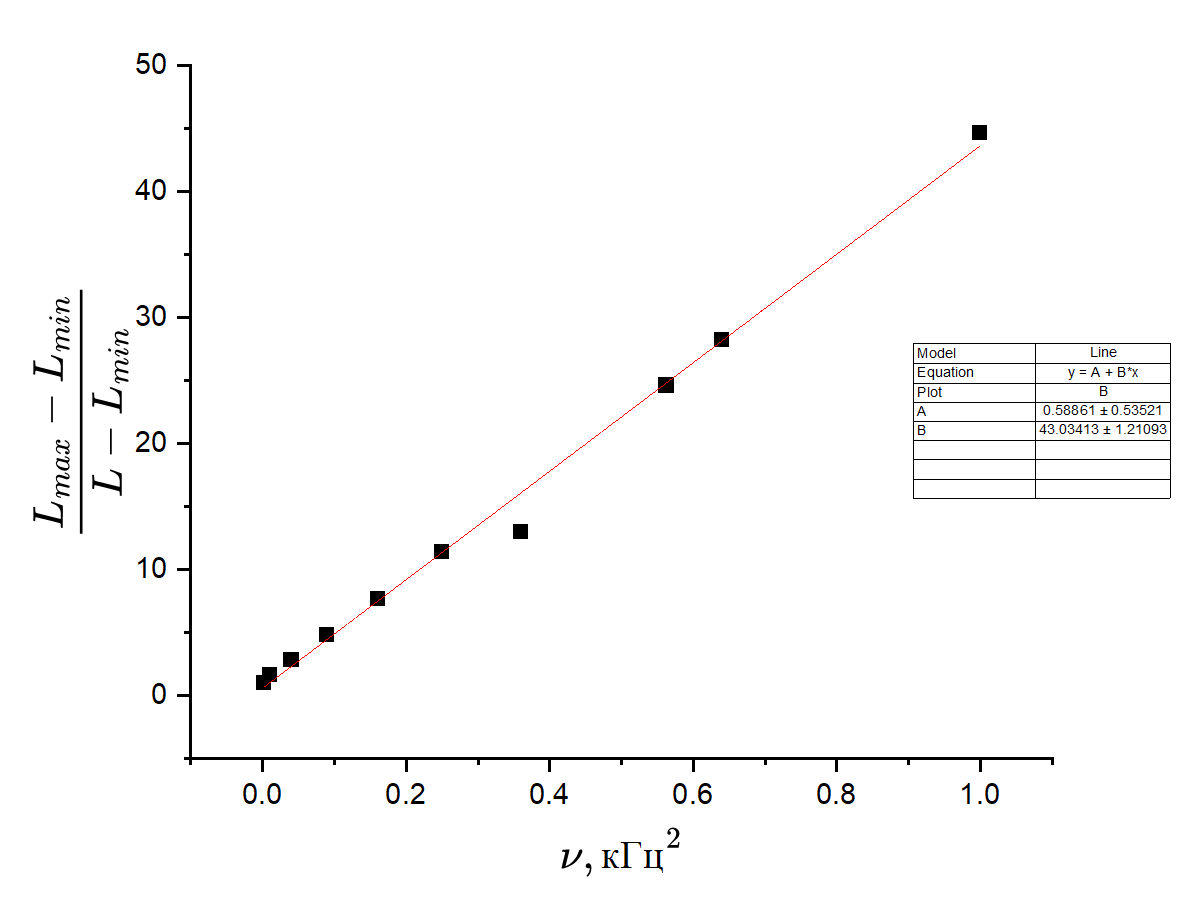
\includegraphics[width=\textwidth]{l.png}}
    \caption{График зависимости $\frac{L_{\max} - L}{L - L_{\min}} (\nu^2)$}\label{fig:L_nu_linearized}
    \newpage
\end{figure}
\begin{equation}
    \sigma = (4.54 \pm 0.27) \cdot 10^7 \text{См/м}
\end{equation}

\newpage
\subsection{Отношение магнитных полей}
Отношение $\abs{H_1}/\abs{H_0}$ можем посчитать двумя способами. Первый способ - через
формулу (\ref{eq:otnoshenie_amplitud}),использовав значение $c$ из пункта (2.1).
Второй способ - через теоретическую формулу (\ref{eq:svyaz_poley}), использовав значение
$\sigma$ из пункта (2.1). Посмотрим на их различие с помощью графиков зависимости
$\abs{H_1}/\abs{H_0} (\nu)$
\begin{figure}[h]
    \center{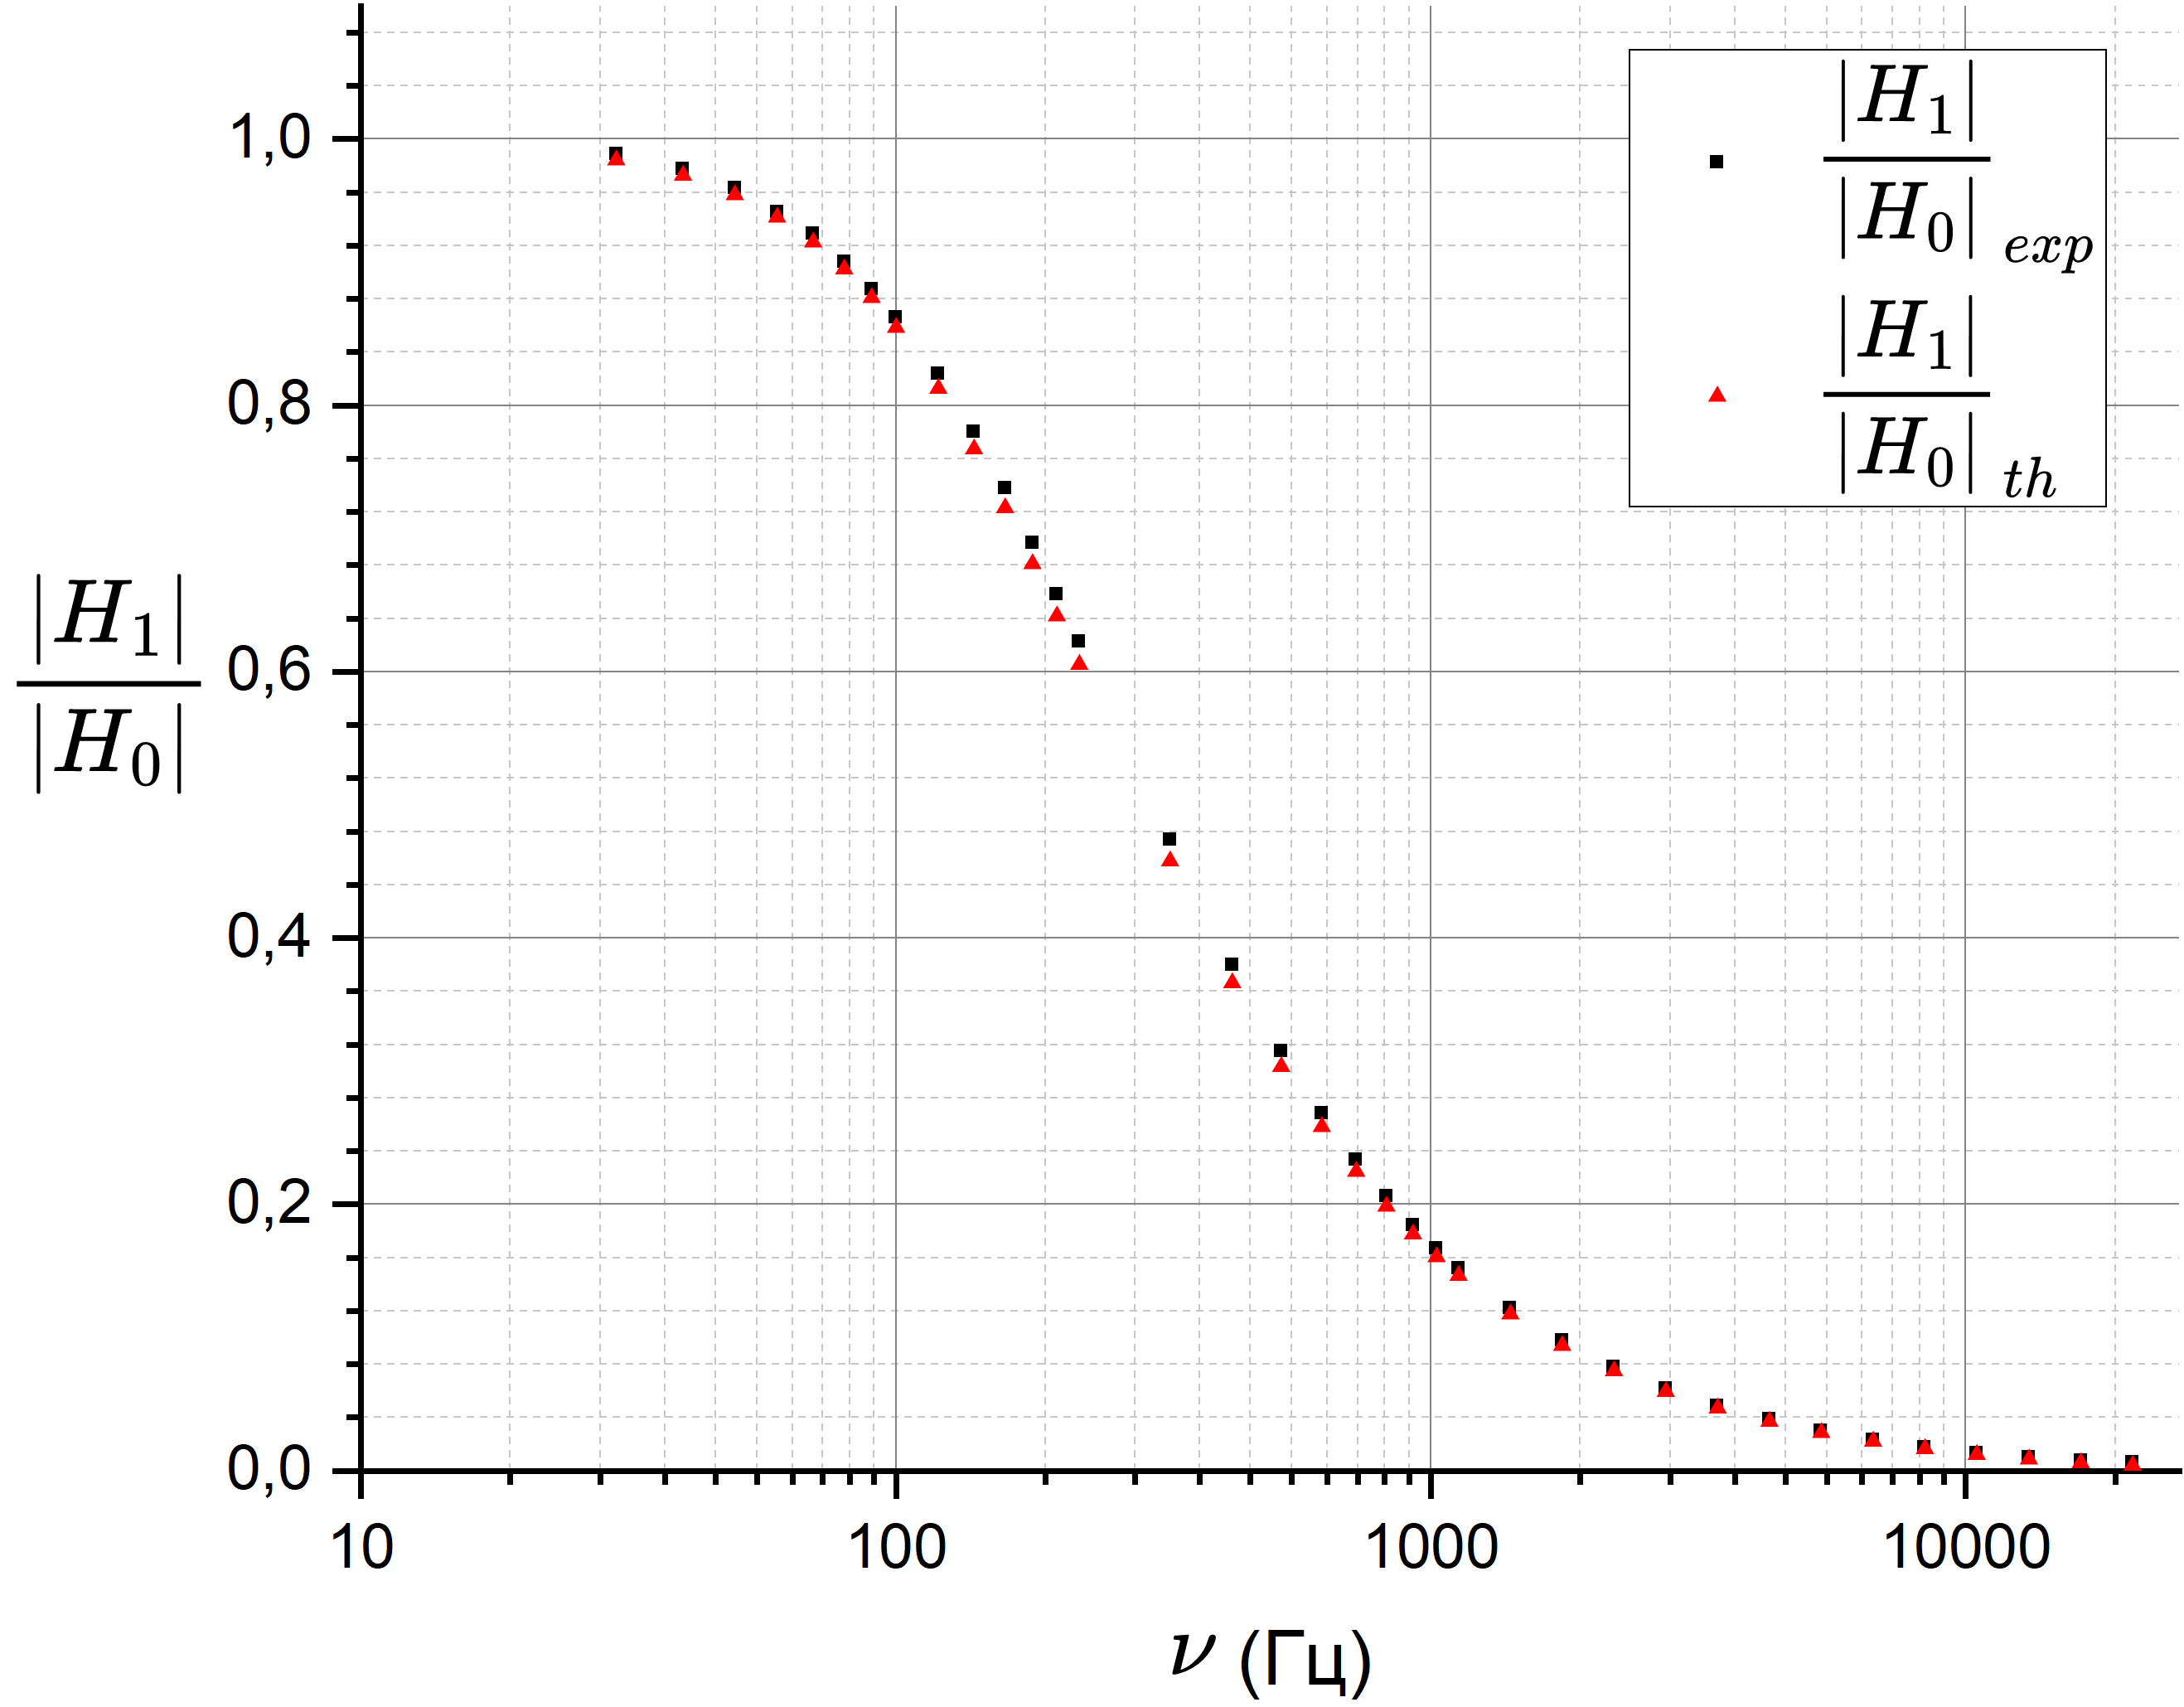
\includegraphics[width=\textwidth]{Final.png}}
    \caption{График зависимости $\frac{H_1}{H_0}(\nu)$}\label{fig:L_nu_linearized}
    \newpage
\end{figure}


\section*{Выводы}
В данной лабораторной работе мы измеряли удельную проводимость меди 4-мя различными способами с помощью явления скин-эффекта. Запишем результаты в общую таблицу:

\begin{table}[!h]
	\begin{center}
		\begin{tabular}{|l|c|c|c|}
			\hline
			Метод измерения & $\sigma, 10^{7} \ \frac{\text{См}}{\text{м}}$ & $\Delta\sigma, 10^{7} \ \frac{\text{См}}{\text{м}}$ & $\varepsilon_{\sigma}$\\
			\hline
			Отношение амплитуд & 4.38 & 0.17 & 3.9\%\\ \hline
			Разности фаз (низкие частоты) & 4.74 & 0.23 & 4.85\%\\ \hline
			Разности фаз (высокие частоты) & 4.28 & 0.33 & 7.71\%\\ \hline
			Индуктивность & 4.54 & 0.27 & 5.94\%\\ \hline
			
		\end{tabular}
	\end{center}
	\caption{Сравнение результатов различных методов}\label{}
\end{table}

В работе использовалась медь марки $M3$, для которой $\sigma_{\text{табл}} = 5.62\cdot10^{7} \ \frac{\text{См}}{\text{м}}$.
Полученные нами значения совпадают по порядку, но, все же, немного нижу табличного значения. Несовпадение может быть вызвано многими факторами, например наводкой поля в соединительных проводах и пренебрежением размерами медного цилиндра и соленоида. 

Методы измерения через разность фаз дали высокие погрешности, потому что измерения делались на глаз на осциллографе, и гарантировать их точность можно только с введенной погрешностью. Кроме того, при измерении на высоких частотах зависимость не является везде линейной, это тоже привносит свою неточность.

Что касается зависимости $\frac{|H_1|}{|H_0|}(\nu)$, то экспериментальные данные очень хорошо согласуются с теоретической зависимостью.
\end{document}